\begin{figure}[ht]
  \centering
  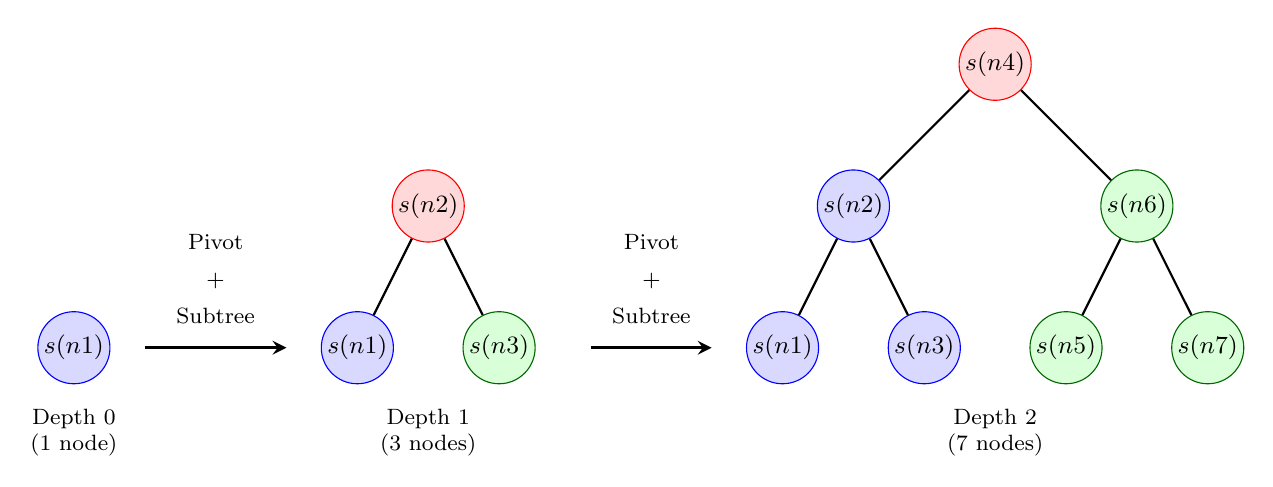
\begin{tikzpicture}[
      scale=.9,
      % The actual tree nodes:
      every node/.style={circle, draw, minimum size=6.5mm, inner sep=1pt, font=\small},
      old/.style={draw=blue, fill=blue!15},
      pivot/.style={draw=red, fill=red!15},
      new/.style={draw=green!40!black, fill=green!15},
      thickedge/.style={draw, thick},
      >=stealth,
      baseline={(current bounding box.south)} % align figure along the bottom
  ]
  
  %%%%%%%%%%%%%%%%%%%%%%%%%%%%%%%%%%%%%%%%%%%%%%%%%%%%%%%%
  % (1) DEPTH=1 => Single node s(n1)
  %%%%%%%%%%%%%%%%%%%%%%%%%%%%%%%%%%%%%%%%%%%%%%%%%%%%%%%%
  \node[old] (A1) at (0,0) {$s(n1)$};
  
  % Depth label below, two lines:
  \node[
    draw=none, fill=none, shape=rectangle, 
    font=\footnotesize, align=center
  ] 
  at (0,-1.2) {Depth 0\\(1 node)};
  
  %%%%%%%%%%%%%%%%%%%%%%%%%%%%%%%%%%%%%%%%%%%%%%%%%%%%%%%%
  % ARROW from first to second
  %%%%%%%%%%%%%%%%%%%%%%%%%%%%%%%%%%%%%%%%%%%%%%%%%%%%%%%%
  \draw[->, very thick] 
    (1,0) -- (3,0)
    node[midway,above=7pt,draw=none,fill=none,shape=rectangle,font=\footnotesize,align=center]
         {Pivot\\[4pt]+\\[4pt]Subtree};
  
  %%%%%%%%%%%%%%%%%%%%%%%%%%%%%%%%%%%%%%%%%%%%%%%%%%%%%%%%
  % (2) DEPTH=2 => 3 nodes total
  %%%%%%%%%%%%%%%%%%%%%%%%%%%%%%%%%%%%%%%%%%%%%%%%%%%%%%%%
  % We'll put old node s(n1) at x=4,y=0
  % pivot s(n2) at x=4,y=2  (2 units above old node)
  % new node s(n3) at x=6,y=0
  
  \node[old]   (Bleft) at (4,0)   {$s(n1)$};
  \node[pivot] (Broot) at (5,2)   {$s(n2)$};
  \draw[thickedge] (Broot) -- (Bleft);
  
  \node[new]   (Bright) at (6,0)  {$s(n3)$};
  \draw[thickedge] (Broot) -- (Bright);
  
  % Depth label below
  \node[
    draw=none, fill=none, shape=rectangle, font=\footnotesize, align=center
  ] 
  at (5,-1.2) {Depth 1\\(3 nodes)};
  
  %%%%%%%%%%%%%%%%%%%%%%%%%%%%%%%%%%%%%%%%%%%%%%%%%%%%%%%%
  % ARROW from second to third
  %%%%%%%%%%%%%%%%%%%%%%%%%%%%%%%%%%%%%%%%%%%%%%%%%%%%%%%%
  \draw[->, very thick]
    (7.3,0) -- (9.0,0)
    node[midway,above=7pt,draw=none,fill=none,shape=rectangle,font=\footnotesize,align=center]
         {Pivot\\[4pt]+\\[4pt]Subtree};
  
  %%%%%%%%%%%%%%%%%%%%%%%%%%%%%%%%%%%%%%%%%%%%%%%%%%%%%%%%
  % (3) DEPTH=3 => 7 nodes total
  %%%%%%%%%%%%%%%%%%%%%%%%%%%%%%%%%%%%%%%%%%%%%%%%%%%%%%%%
  % We'll keep old node s(n1) at (10,0)
  % old pivot s(n2) at (10,2)
  % new pivot s(n4) at (10,4)
  % old right node s(n3) at (12,0)
  % new subtree root s(n5) at (12,2)
  % leaves s(n6) at (11.5,0) and s(n7) at (12.5,0)
  
  \node[old]   (ColdLeft)  at (10,0) {$s(n1)$};
  \node[old]   (ColdRoot)  at (11,2) {$s(n2)$};
  \draw[thickedge] (ColdRoot) -- (ColdLeft);
  
  \node[pivot] (Croot)     at (13,4) {$s(n4)$};
  \draw[thickedge] (Croot) -- (ColdRoot);
  
  \node[old]   (ColdRight) at (12,0) {$s(n3)$};
  \draw[thickedge] (ColdRoot) -- (ColdRight);
  
  \node[new]   (CrightRoot) at (15,2) {$s(n6)$};
  \draw[thickedge] (Croot) -- (CrightRoot);
  
  \node[new]   (CrightL)   at (14,0) {$s(n5)$};
  \node[new]   (CrightR)   at (16,0) {$s(n7)$};
  
  \draw[thickedge] (CrightRoot) -- (CrightL);
  \draw[thickedge] (CrightRoot) -- (CrightR);
  
  % Depth label for third tree, two lines
  \node[
    draw=none, fill=none, shape=rectangle,
    font=\footnotesize, align=center
  ] 
  at (13,-1.2) {Depth 2\\(7 nodes)};
  
  \end{tikzpicture}
  
  \caption{From left (Depth 0) to right (Depth 2), illustrating meltdown-free expansions:
  old nodes (blue) at the bottom, pivot node(s) (red) placed above,
  and any new subtree nodes (green) at the bottom again. 
  We space each depth label on two lines below the tree, 
  and put line breaks in the arrow labels as well.}
  \label{fig:geosodic-expansion}
  \end{figure}
  